\section{Fase di progettazione}
\label{sec:fase_di_progettazione}
\subsection{Struttura}
\label{sub:struttura}
\subsubsection{Header}
\label{ssub:header}
L'header contiene logo, nav, breadcrumb e due link per il login e il signup. Il logo, situato in alto a sinistra, non rimanda a nessuna pagina in quanto il link per la homepage è già contenuto nel menu sotto la voce Home. I due pulsanti per il login e il signup sono rispettivamente ``Accedi'' e ``Registrati'' e sono entrambi presenti solo nel caso in cui l'utente non abbia ancora effettuato l'accesso. Una volta effettuato l'accesso, al posto dei due link c'è il nickname dell'utente e il link ``esci'' che scollega l'utente e lo porta alla home.
% subsubsection header (end)
\paragraph{Nav}
\label{par:nav}
Il nav del sito contiene il menu e la barra di ricerca.
Il menu occupa la posizione centrale dell'header e contiene i link alle pagine principali del sito:
\begin{itemize}
	\item Home page;
	\item Pagina relativa ai primi piatti;
	\item Pagina relativa ai secondi piatti;
	\item Pagina relativa ai dolci;
\end{itemize}
La barra di ricerca è situata sotto il menu in posizione centrale ed è ben visibile per permettere agli utenti di cercare le ricette di cui hanno bisogno.
% paragraph nav (end)
\paragraph{Breadcrumb}
\label{par:breadcrumb}
Il breadcrumb è posizionato a sinistra sotto la barra di ricerca e serve a identificare la posizione dell'utente all'interno del sito. L'ultimo campo corrisponde alla pagina corrente e, per evitare link circolari, è un testo.
% paragraph breadcrumb (end)
\subsubsection{Content}
\label{ssub:content}
Lo scopo principale del sito è cercare e consultare le ricette a cui si è interessati.

\paragraph{Pagina Home}
È la prima pagina ad essere visualizzata quando un utente visita il sito, contiene una breve descrizione dei contenuti.
Sono poi presenti le tre ricette (una per portata) con il voto più alto.

\paragraph{Pagine delle portate}
Le pagine con gli elenchi dei primi piatti, i secondi piatti e i dolci hanno la stessa struttura: in ogni pagina viene presentata la lista di tutte le ricette relative alla portata selezionata. Le ricette sono presentate in riquadri contenenti l'immagine del piatto, il nome, la difficoltà, il tempo necessario allo svolgimento, il voto medio e il link ``apri'' che porta alla pagina della ricetta selezionata.

\paragraph{Pagine delle ricette}
È la pagina in cui viene presentata la ricetta selezionata. Per prima cosa, è visibile il titolo della ricetta, l'immagine del piatto e sulla destra la lista degli ingredienti, la difficoltà e la durata della ricetta; in seguito è descritto il procedimento, seguito da un form che permette di assegnare alla ricetta un voto da 1 a 5. Infine c'è la sezione dei commenti in cui è possibile inserire un commento relativo alla ricetta e leggere i commenti degli altri utenti.

\paragraph{Pagine di Login e Signup}
L'utente ha la possibilità di registrarsi o accedere con le proprie credenziali tramite le pagine di login e signup. Nella pagina signup sono presenti dei campi per inserire l'indirizzo email, il nickname e la password (quest'ultima da inserire due volte per confermare la correttezza). Per il login è necessario inserire  il nickname e la password.

\paragraph{Pagina Utente}
Una volta effettuato l'accesso, l'utente può visitare la propria area personale e verificare le proprie informazioni correnti. C'è la possibilità di eliminare l'account inserendo la propria password nel form apposito in fondo alla pagina.

\paragraph{Pagina Modifica Utente}
Dalla pagina utente è possibile aprire la pagina modifica utente in cui sono presenti tutti i form necessari per cambiare le informazioni dell'utente (immagine, nickname, email e password). Ciascun form permette la modifica di un unica informazione, e deve essere confermato inserendo la password attuale. Nel caso si vogliano annullare le modifiche, lo si può fare mediante il pulsante ``Annulla'', in fondo alla pagina.

\paragraph{Pagine Aggiungi e Modifica ricetta}
Queste pagine sono raggiungibili solo dagli utenti con permessi amministratore. In entrambe le pagine sono presenti i form per l'inserimento delle informazioni che poi compariranno nella pagina della ricetta. Nella pagina ``modifica ricetta'' i form sono già compilati con le informazioni attuali. Anche in questo caso, per annullare le modifiche è presente il pulsante ``Annulla'' in fondo alla pagina.

% subsubsection content (end)
\subsubsection{Footer}
\label{ssub:footer}
Il footer contiene la dicitura per il copyright, i nomi degli autori del sito, e le icone di certificazione della validità rispetto agli standard W3C di XHTML e CSS3.

% subsubsection footer (end)
% subsection struttura (end)
\subsection{Visualizzazione} %le pagine devono essere accessibili indipendentemente dalle dimensioni del dispositivo e del browser
\label{sub:visualizzazione}
La visualizzazione del sito è stata pensata in modo da rendere le pagine accessibili ad ogni categoria di utente e reattive alla tipologia di dispositivo utilizzato. Sono state quindi utilizzate unità di misura relative e colori che garantissero sempre un adeguato livello di contrasto tra le scritte e lo sfondo sottostante. \\
Sono state previste quattro tipologie di visualizzazione del sito: desktop, tablet, mobile e stampa.
\subsubsection{Desktop}
\label{ssub:desktop}
Nella visualizzazione desktop il layout è diviso in tre schede posizionate vericalmente. La prima presenta il logo del sito, i link per effettuare l'accesso e la registrazione, il menù e la barra di ricerca. In questo modo appena l'utente entra nel sito può facilmente raggiungere la pagina desiderata. \\
La seconda scheda racchiude il contenuto che si adatta in base alla grandezza della schermata, in particolare gli elenchi delle ricette mostreranno da 1 a 3 ricette per fila dipendentemente dallo spazio a disposizione. \\
La terza scheda contiene infine il footer.  
\begin{figure}[H]
	\centering
	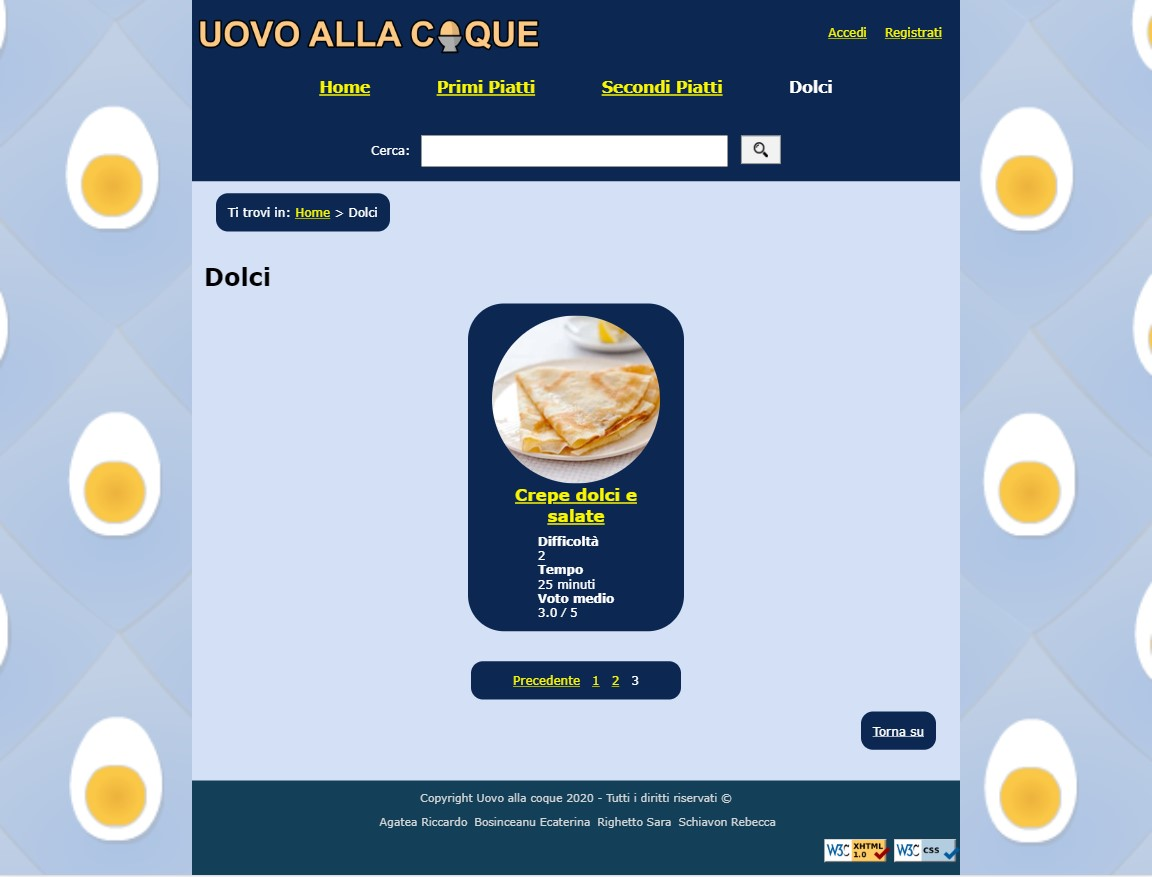
\includegraphics[width=16cm]{img/progettazione/desktop.jpg}
\end{figure}
% subsubsection desktop (end)
\subsubsection{Tablet}
\label{ssub:tablet}
La visualizzazione tablet è pensata per dispositivi con meno spazio rispetto al desktop e per questo motivo lo spazio dedicato alla prima scheda viene visibilmente ridimensionato passando da un menù sempre visibile ad un menù ad hamburger, in cui è necessario premere l'apposito pulsante, in questo caso situato in alto a destra, per farlo apparire. Una volta aperto, il menù occupa la parte destra dello schermo e presenta le varie voci in verticale. Sono presenti inoltre i link per il login e il signup e la barra di ricerca posizionata sul fondo del menù. Si è deciso di inserire tutte le voci insieme alla barra di ricerca nel menù, per avere tutti gli elementi necessari per la navigazione raccolti in un unico spazio. Quando il menù è chiuso è visibile solo il logo affiancato dal tasto del menù. \\
Il resto del design resta, invece, invariato.

\begin{figure}[H]
	\begin{minipage}[b]{8.5cm}
		\centering
		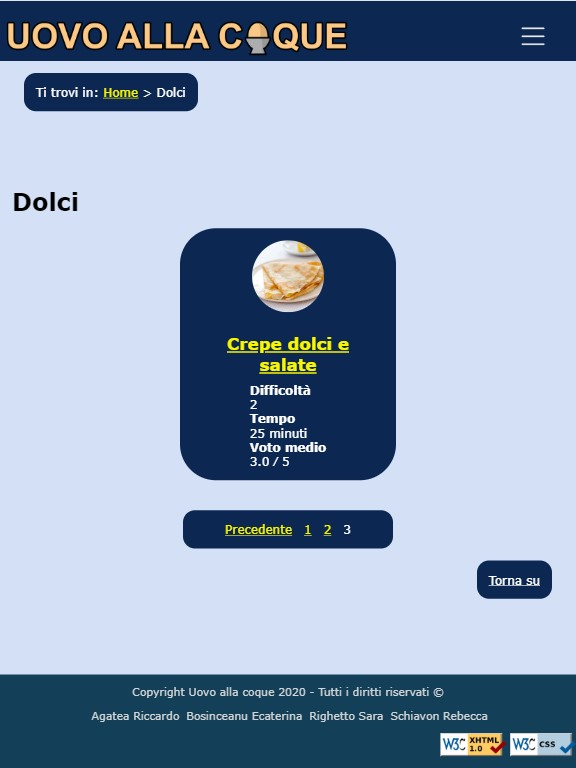
\includegraphics[width=8cm]{img/progettazione/tablet.jpg}
		\caption{Pagina con la visualizzazione tablet}
	\end{minipage}
	\ \hspace{2mm} \hspace{3mm} \
	\begin{minipage}[b]{8.5cm}
		\centering
		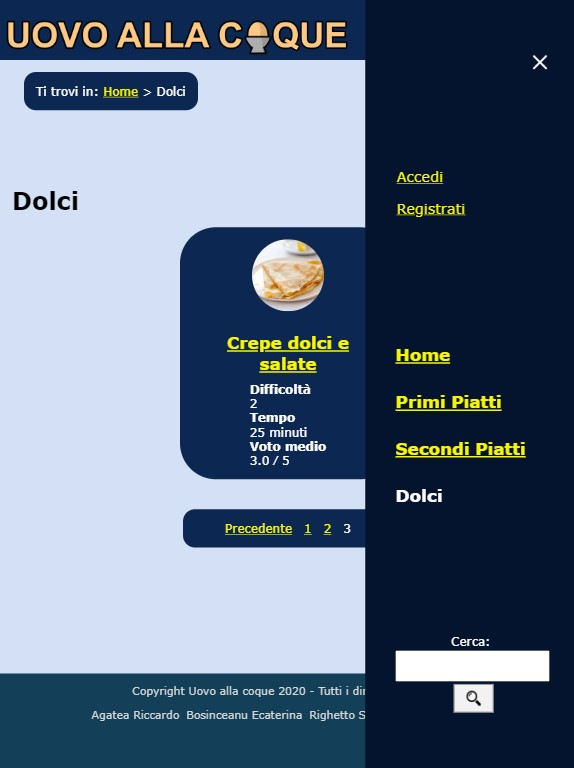
\includegraphics[width=8cm]{img/progettazione/tablet-menu.jpg}
		\caption{Menù hamburger in tablet}
	\end{minipage}
\end{figure}

% subsubsection tablet (end)
\subsubsection{Mobile}
\label{ssub:mobile}
Anche nella visualizzazione da mobile è stato implementato il menù ad hamburger al fine di gestire al meglio lo spazio disponibile. Il pulsante è facilmente raggiungibile per gli utenti che usano il telefono con due mani, mentre gli utenti destri che usano il telefano con una sola mano potranno aprire comodamente il menù col pollice. Una volta aperto, occupa quasi tutto lo schermo.
\begin{figure}[H]
	\begin{minipage}[b]{8.5cm}
		\centering
		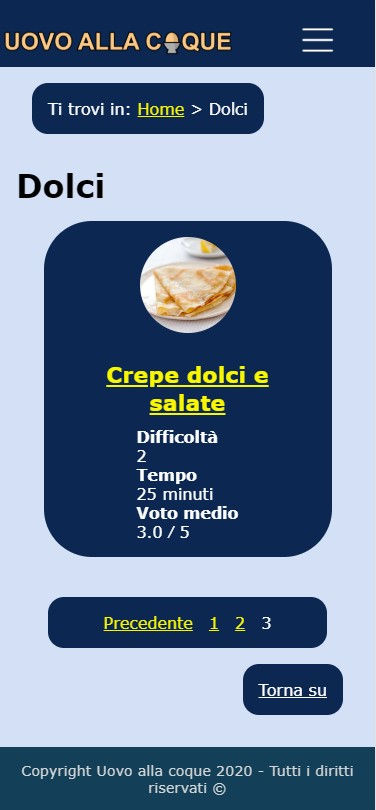
\includegraphics[width=8cm]{img/progettazione/mobile.jpg}
		\caption{Pagina con la visualizzazione mobile}
	\end{minipage}
	\ \hspace{2mm} \hspace{3mm} \
	\begin{minipage}[b]{8.5cm}
		\centering
		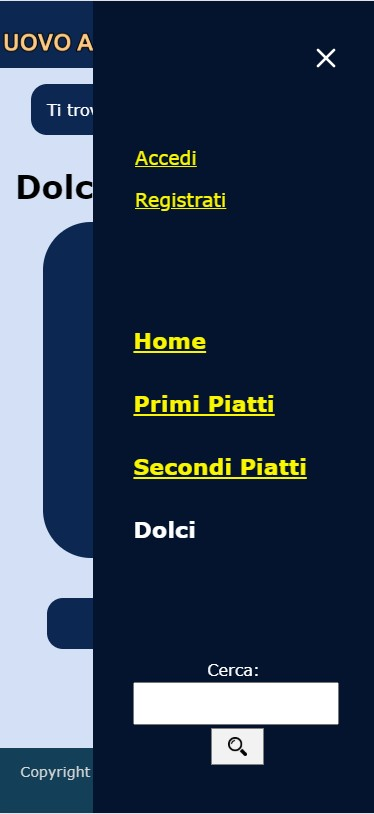
\includegraphics[width=8cm]{img/progettazione/mobile-menu.jpg}
		\caption{Menù hamburger in mobile}
	\end{minipage}
\end{figure}


% subsubsection mobile (end)
\subsubsection{Stampa}
\label{ssub:stampa}
Per quanto riguarda la stampa, sono stati eliminati gli elementi di presentazione (immagini e background) e sono stati tenuti solo gli elementi necessari, ovvero il contenuto della pagina. È stato rimosso il menù, la barra di ricerca e il footer in quanto non necessari per la visualizzazione della pagina stampata, mentre sono stati tenuti il breadcrumb per specificare il percorso alla pagina selezionata, e il logo per distinguere il sito.
Le pagine sono in bianco e nero per dare valore al contenuto anzichè alla presentazione. Il font, che nella visualizzazione a schermo era san-serif, passa ad essere serif per una migliore leggibilità sulla carta stampata.
% subsubsection stampa (end)
% subsection visualizzazione (end)

\subsection{Accessibilità}
\label{sub:accessibilità}
Per garantire un alto livello di accessibilità sono state le linee guida dello standard WCAG. Comportamento, struttura e presentazione sono separate per permettere un miglior accesso al sito tramite diversi motori di ricerca e browser, inoltre, facilita l'interazione con utenti che presentano disabilità.

\subsubsection{Comportamento}
Il sito offre la possibilità di cercare ricette in modo preciso tramite la barra di ricerca, altrimenti, le ricette più votate presenti nella home rappresentano uno spunto per esplorare le ricette all'interno del sito. La suddivisione delle ricette tra le pagine dei primi, secondi e dolci facilitano l'esplorazione del sito e una ricerca più mirata. Le informazioni sono reperibili con un numero limitato di click: ad esempio per accedere ad una determinata ricetta cercata tramite la barra di ricerca, saranno sufficienti due click.
Per facilitare la navigazione, sul fondo di ogni pagina c'è il pulsante "torna su" che permette di raggiungere l'inizio della pagina senza utilizzare lo scroll. Inoltre, in ogni pagina è presente il breadcrumb che mostra la posizione dell'utente all'interno del sito. I link circolari vengono evitati rendendo l'ultimo campo del breadcrumb (che rappresenta la pagina corrente) semplice testo; lo stesso vale per tutti i link presenti nel header: una volta raggiunta una certa pagina, il link corrispondente non sarà clickabile perchè sarà testo.
I tag input sono sottoposti ad un processo di validazione per garantire il corretto inserimento dei dati richiesti. Nel caso un input non superi la validazione, viene mostrato un messaggio di errore che spiega l'errore commesso ed eventualmente come si può evitare. Il messaggio di errore non elimina il contenuto dei tag, per permettere all' utente di modificare i dati senza risciverli.

\subsubsection{Struttura}
% tutte le immagini hanno specificato la proprietà alt
% utilizzare label per element del form, in modo da facilitate gli screen reader (fieldset)
% non c'è testo libero, tutto è incapsulato dentro ad appositi tag descrittivi
% Usare Access Key per i comandi rapidi alle funzioni principali.
% Ogni link deve avere un'ancora diversa per evitare link che portano alla stessa pagina.
% Esplicitare acronimi di abbreviazioni e sigle per screen reader e motori ricerca.
% Tenere sempre presente il "Dove sono", "Da dove sono venuto" e "Dove posso andare".

\subsubsection{Presentazione}
Tramite il CSS è stato implementato il design utilizzando classi che definiscono il contenuto dell'oggetto e non il comportamento, in modo da mantenere la separazione tra comportamento e presentazione. Vengono utilizzate misure relative (em) o in percentuale per permettere una corretta visualizzazione delle pagine su schermi di dimensioni diverse. Sono presenti due fogli di stile diversi: il primo è dedicato alla stampa mentre il secondo è dedicato alla visualizzazione da dasktop e mobile.
Il colore dominante del sito è il blu: il background è un pattern con le uova a sfondo azzurro, a contrasto col header e gli elementi del sito color blu scuro. Le scritte sono bianche per essere in contrasto col blu, oppure gialle nel caso dei link visitati.Il colore utilizzato per l' hover dei link è in contrasto sia con lo sfondo che col colore della scritta. Il rapporto tra colore di sfondo e testo superano il test WCAG AAA che richiede un rapporto di contrasto di almeno 7:1 per il testo normale e 4.5:1 per il testo in grassetto.

% come da specifiche è stata rispettata la completa separazione tra comportamento, presentazione e struttura.
% ricerca: già scritta nell analisi
% torna su: poichè il menu sia nella visualizzazione desktop che quella mobile, è fisso all'inizio di ogni pagina, per raggiungerlo facilmente dopo uno scroll verticale, sono stati posizionati delle ancore "torna su", che rimandano all' header della pagina attuale.
% il logo nell'header non rimanda alla home
% Dare le informazioni con un numero limitato di click: con solo due click si può accedere ad una ricetta, per esempio Primi piatti > Carbonara. 
% Non obbligare utente e reinserire i campi dei form dopo messaggi di errore. -> session di php
% Ogni messaggio di errore deve essere corredato da "che errore è" e da "Come fare a risolvere". validazione php js


% \subsubsection{Convenzioni interne}
% \label{ssub:convenzioni_interne}
% Una delle convenzioni interne al sito riguarda i link: sono sottolineati per permettere l'immediata individuazione, e quelli visitati diventano gialli. % non ci sono link circolari. Quando sei loggato, il registrati nel contenuto della home non è più cliccabile
% subsubsection convenzioni_interne (end)
% fare riferimento al w3c https://www.w3.org/standards/webdesign/accessibility
% subsection accessibilità (end)

% section fase_di_progettazione (end)
